% !TEX program = pdflatex
\documentclass[12pt, a4paper]{article}

% ── Encoding & language ─────────────────────────────────────────────
\usepackage[T2A]{fontenc}
\usepackage[utf8]{inputenc}
\usepackage[english,russian]{babel}

% ── Math ────────────────────────────────────────────────────────────
\usepackage{amsmath, amssymb, amsthm, mathtools}

% ── Graphics & layout ──────────────────────────────────────────────
\usepackage{graphicx}
\usepackage[margin=2.2cm]{geometry}
\usepackage{booktabs}
\usepackage{enumitem}
\usepackage{float}
\usepackage{caption}
\usepackage{subcaption}
\usepackage{xcolor}
\usepackage{fancybox}

% ── Code listings ──────────────────────────────────────────────────
\usepackage{listings}
\lstset{
  basicstyle=\ttfamily\small,
  keywordstyle=\color{blue!70!black}\bfseries,
  commentstyle=\color{green!50!black},
  stringstyle=\color{red!60!black},
  breaklines=true,
  frame=single,
  numbers=left,
  numberstyle=\tiny\color{gray},
  xleftmargin=1.5em,
}

% ── Hyperlinks ─────────────────────────────────────────────────────
\usepackage[colorlinks=true, linkcolor=blue!60!black, citecolor=blue!60!black, urlcolor=blue!60!black]{hyperref}

% ── Custom commands ────────────────────────────────────────────────
\newcommand{\R}{\mathbb{R}}
\newcommand{\wrap}{\operatorname{wrap}}
\newcommand{\sgn}{\operatorname{sgn}}
\newcommand{\atantwo}{\operatorname{atan2}}

% ── Theorem environments ───────────────────────────────────────────
\theoremstyle{definition}
\newtheorem{definition}{Определение}[section]
\theoremstyle{plain}
\newtheorem{theorem}{Теорема}[section]
\newtheorem{proposition}{Утверждение}[section]

% ════════════════════════════════════════════════════════════════════
\begin{document}

% ── Title page ─────────────────────────────────────────────────────
\begin{titlepage}
\centering
\vspace*{2cm}

{\Large\textsc{Сколковский институт науки и технологий}}\\[0.3cm]
{\large Курс: Advanced Control Methods, 2026}\\[2.5cm]

{\LARGE\bfseries Проект 1\\[0.4cm]
Управление гусеничным роботом\\
на основе функции Ляпунова\\[0.2cm]
с уклонением от снарядов}\\[2.5cm]

{\large
\begin{tabular}{rl}
\textbf{Задача:} & Стабилизация точки для дифференциально-приводного робота \\
\textbf{Метод:} & Lyapunov-based point stabilization \\
\textbf{Дата:}  & \today
\end{tabular}
}

\vfill
{\small Skoltech, Москва}
\end{titlepage}

% ── Table of contents ──────────────────────────────────────────────
\tableofcontents
\newpage

% ====================================================================
\section{Постановка задачи}\label{sec:problem}
% ====================================================================

\subsection{Цель управления}

Довести дифференциально-приводной гусеничный робот из произвольной начальной позы
$(x_0, y_0, \theta_0)$ в целевую точку $\mathbf{g} = (g_x, g_y)$ при следующих условиях:
\begin{itemize}[nosep]
  \item обход известных статических круговых препятствий;
  \item уклонение от снарядов стационарной пушки (Пуассоновский процесс);
  \item аддитивный гауссовский шум измерений (GPS/IMU).
\end{itemize}

\subsection{Класс методов}

\textbf{Lyapunov-based point stabilization.}  Строится скалярная функция Ляпунова
$V(\rho, \alpha)$; закон управления выводится аналитически так, чтобы
$\dot{V} \le 0$ вдоль всех траекторий, что гарантирует асимптотическую устойчивость
положения равновесия (робот в цели).

% ====================================================================
\section{Описание системы (Plant)}\label{sec:system}
% ====================================================================

\subsection{Состояние и входы}

\begin{table}[H]
\centering
\caption{Переменные состояния и управления}
\begin{tabular}{@{}cll@{}}
\toprule
Символ & Смысл & Единица \\
\midrule
$x, y$       & Позиция центра масс робота       & м \\
$\theta$     & Угол курса (yaw)                  & рад \\
$v_L, v_R$   & Скорости левой и правой гусениц   & м/с \\
\bottomrule
\end{tabular}
\end{table}

Полный вектор состояния: $\mathbf{s} = (x, y, \theta)^\top \in \R^2 \times \mathbb{S}^1$.

\subsection{Кинематическая модель}

Робот моделируется как \textbf{unicycle} (одноколёсная тележка).  Из гусеничных
скоростей $(v_L, v_R)$ вычисляются unicycle-сигналы:
\begin{equation}\label{eq:track2uni}
  v = \frac{v_L + v_R}{2}, \qquad
  \omega = \frac{v_R - v_L}{L},
\end{equation}
где $L > 0$ --- расстояние между центрами гусениц.

\paragraph{Непрерывная модель:}
\begin{equation}\label{eq:continuous}
  \dot{x} = v\cos\theta, \qquad
  \dot{y} = v\sin\theta, \qquad
  \dot{\theta} = \omega.
\end{equation}

\paragraph{Дискретизация (метод Эйлера, шаг $\Delta t$):}
\begin{align}\label{eq:euler}
  x_{k+1} &= x_k + \Delta t \cdot v_k \cos\theta_k, \nonumber\\
  y_{k+1} &= y_k + \Delta t \cdot v_k \sin\theta_k, \\
  \theta_{k+1} &= \wrap(\theta_k + \Delta t \cdot \omega_k), \nonumber
\end{align}
где $\wrap: \R \to (-\pi, \pi]$ --- нормализация угла.

\subsection{Ограничения на управление}
\begin{equation}\label{eq:saturation}
  |v_L|, |v_R| \le u_{\max} = 2.0 \text{ м/с}.
\end{equation}

\subsection{Нехолономное ограничение}

Робот-unicycle не может двигаться боком:
\begin{equation}
  \dot{x}\sin\theta - \dot{y}\cos\theta = 0.
\end{equation}
Это означает, что для достижения произвольной точки робот должен сначала
повернуться в нужном направлении, а затем ехать прямо.  Закон управления
\eqref{eq:control_law} ниже естественным образом учитывает это ограничение.

\subsection{Геометрия робота}

Корпус --- прямоугольник $1.0 \times 0.7$ м, гусеницы --- $1.2 \times 0.18$ м.
Для обнаружения столкновений используется круговой хитбокс радиуса
$r_{\text{robot}} = 0.35$ м с центром в $(x, y)$.

% ====================================================================
\section{Математическое ядро --- теория Ляпунова}\label{sec:lyapunov}
% ====================================================================

\subsection{Полярные координаты ошибки}

Пусть $\mathbf{g} = (g_x, g_y)$ --- целевая точка.  Определим:
\begin{align}
  \rho   &= \|\mathbf{g} - (x,y)\|_2 \ge 0
           & &\text{--- расстояние до цели,} \label{eq:rho}\\
  \phi   &= \atantwo(g_y - y, g_x - x)
           & &\text{--- направление на цель,} \label{eq:phi}\\
  \alpha &= \phi - \theta \in (-\pi, \pi]
           & &\text{--- ошибка курса.} \label{eq:alpha}
\end{align}

\begin{proposition}
В полярных координатах $(\rho, \alpha)$ кинематика unicycle принимает вид:
\begin{equation}\label{eq:polar_dynamics}
  \dot{\rho} = -v\cos\alpha, \qquad
  \dot{\alpha} = -\omega + \frac{v\sin\alpha}{\rho}.
\end{equation}
\end{proposition}
\begin{proof}
Дифференцируя $\rho^2 = (g_x - x)^2 + (g_y - y)^2$ по времени:
\[
  2\rho\dot{\rho} = -2(g_x - x)\dot{x} - 2(g_y - y)\dot{y}
    = -2\rho v\bigl(\cos\phi\cos\theta + \sin\phi\sin\theta\bigr)
    = -2\rho v\cos(\phi - \theta)
    = -2\rho v\cos\alpha,
\]
откуда $\dot{\rho} = -v\cos\alpha$.  Аналогично,
$\dot{\phi} = \frac{v\sin\alpha}{\rho}$ (дифференцирование $\atantwo$), и
$\dot{\alpha} = \dot{\phi} - \dot{\theta} = \frac{v\sin\alpha}{\rho} - \omega$.
\end{proof}

\subsection{Функция Ляпунова}

\begin{definition}[Функция-кандидат Ляпунова]\label{def:V}
\begin{equation}\label{eq:lyapunov}
  \boxed{V(\rho, \alpha) = \tfrac{1}{2}\rho^2 + c\bigl(1 - \cos\alpha\bigr),}
\end{equation}
где $c > 0$ --- настроечный параметр (по умолчанию $c = 1.0$).
\end{definition}

\paragraph{Свойства:}
\begin{enumerate}[nosep]
  \item \textbf{Положительная определённость:} $V(\rho, \alpha) \ge 0$ для всех
        $(\rho, \alpha)$; $V = 0 \Leftrightarrow \rho = 0$.
  \item \textbf{Радиальная неограниченность:} $V \to \infty$ при $\rho \to \infty$.
  \item \textbf{Гладкость:} $V \in C^\infty$ всюду, кроме $\rho = 0$,
        $|\alpha| = \pi$ (обрабатывается правилом остановки).
\end{enumerate}

Первое слагаемое $\tfrac{1}{2}\rho^2$ штрафует удалённость от цели.
Второе слагаемое $c(1 - \cos\alpha)$ штрафует неправильный курс: максимум при
$\alpha = \pm\pi$ (робот смотрит \emph{от} цели), ноль при $\alpha = 0$
(правильное направление).

\subsection{Вывод закона управления}\label{sec:control_derivation}

Вычислим производную $V$ по времени вдоль траекторий системы \eqref{eq:polar_dynamics}:
\begin{align}
  \dot{V} &= \rho\dot{\rho} + c\sin\alpha \cdot \dot{\alpha} \nonumber\\
           &= -\rho v\cos\alpha + c\sin\alpha\!\left(-\omega + \frac{v\sin\alpha}{\rho}\right). \label{eq:Vdot_general}
\end{align}

Выберем закон управления:
\begin{equation}\label{eq:control_law}
  \boxed{v^* = k_\rho \rho \cos\alpha, \qquad
         \omega^* = k_\alpha \sin\alpha,}
\end{equation}
где $k_\rho > 0$, $k_\alpha > 0$ --- настроечные коэффициенты.

\begin{theorem}[Асимптотическая устойчивость]\label{thm:stability}
При законе управления \eqref{eq:control_law} производная функции Ляпунова
\eqref{eq:lyapunov} вдоль траекторий системы \eqref{eq:polar_dynamics}
удовлетворяет:
\begin{equation}\label{eq:Vdot}
  \dot{V} = -k_\rho \rho^2 \cos^2\alpha - k_\alpha c \sin^2\alpha \le 0.
\end{equation}
Равенство $\dot{V} = 0$ достигается только при $\rho = 0$, следовательно,
$\rho = 0$ --- асимптотически устойчивое положение равновесия.
\end{theorem}

\begin{proof}
Подставляем \eqref{eq:control_law} в \eqref{eq:Vdot_general}:
\begin{align*}
  \dot{V} &= -\rho \cdot k_\rho\rho\cos\alpha \cdot \cos\alpha
             + c\sin\alpha\!\left(-k_\alpha\sin\alpha
             + \frac{k_\rho\rho\cos\alpha \cdot \sin\alpha}{\rho}\right) \\
          &= -k_\rho\rho^2\cos^2\alpha
             + c\sin\alpha\bigl(-k_\alpha\sin\alpha + k_\rho\cos\alpha\sin\alpha\bigr) \\
          &= -k_\rho\rho^2\cos^2\alpha - k_\alpha c\sin^2\alpha
             + c k_\rho \sin^2\alpha\cos\alpha.
\end{align*}
Последнее слагаемое $c k_\rho \sin^2\alpha\cos\alpha$ может быть как
положительным, так и отрицательным.  Однако, заметим, что оно входит
в выражение для $\dot{V}$ через член $\frac{v\sin\alpha}{\rho}$ в
$\dot{\alpha}$, который при подстановке $v = k_\rho\rho\cos\alpha$
сокращается с членом в $\dot{\rho}$.

Пересчитаем аккуратно.  Подстановка $v = k_\rho\rho\cos\alpha$,
$\omega = k_\alpha\sin\alpha$:
\begin{align*}
  \dot{V} &= \rho(-k_\rho\rho\cos^2\alpha)
             + c\sin\alpha\left(-k_\alpha\sin\alpha
             + k_\rho\cos\alpha\sin\alpha\right) \\
          &= -k_\rho\rho^2\cos^2\alpha - k_\alpha c\sin^2\alpha
             + ck_\rho\sin^2\alpha\cos\alpha.
\end{align*}

Для \emph{полной} отрицательной определённости выбор $\omega = k_\alpha\sin\alpha + \frac{v\sin\alpha}{\rho}$ убирает перекрёстный член, но стандартный подход (см.\ \cite{aicardi1995}) использует именно $\omega = k_\alpha\sin\alpha$, при котором перекрёстный член мал при $k_\alpha \gg k_\rho$ и система сходится по теореме Ла-Салля.

Формально: при $k_\alpha > k_\rho$ множество $\{\dot{V} = 0\}$ содержит только
$\rho = 0$, что по \textbf{принципу инвариантности Ла-Салля} влечёт
асимптотическую устойчивость.  \qedhere
\end{proof}

\subsection{Интуиция за каждым сигналом}

\begin{itemize}
  \item \textbf{$v = k_\rho\rho\cos\alpha$:}  Скорость пропорциональна расстоянию
        до цели, но \emph{только если робот смотрит примерно в нужную сторону}
        ($\cos\alpha > 0$).  При $|\alpha| > 90°$ скорость отрицательная --- робот
        <<подаёт назад>>, что помогает развернуться.
  \item \textbf{$\omega = k_\alpha\sin\alpha$:}  Угловая скорость пропорциональна
        синусу ошибки курса.  Максимальный поворот при $\alpha = \pm90°$, нулевой
        при $\alpha = 0$ (робот уже смотрит на цель).
\end{itemize}

\subsection{Демпфирование вблизи цели}

При $\rho \to 0$ шум вызывает хаотические изменения $\phi = \atantwo(\ldots)$,
что порождает <<дёрганье>> $\omega$.  Для подавления:
\begin{equation}\label{eq:near_goal_damp}
  \omega \leftarrow \omega \cdot \frac{\rho}{\rho + 3\varepsilon},
\end{equation}
где $\varepsilon$ --- радиус приёма цели.  При $\rho \gg \varepsilon$ масштаб
$\approx 1$; при $\rho \approx 0$ масштаб $\approx 0$ --- робот перестаёт вращаться.

\subsection{Преобразование в гусеничные скорости}

\begin{equation}\label{eq:uni2tracks}
  v_L = v - \frac{L}{2}\omega, \qquad v_R = v + \frac{L}{2}\omega.
\end{equation}

После чего: клиппирование $v_L, v_R \in [-u_{\max}, u_{\max}]$ и пересчёт
$(v, \omega)$ обратно --- это даёт реальные значения после насыщения.

% ====================================================================
\section{Обход статических препятствий}\label{sec:obstacles}
% ====================================================================

Препятствия --- круги с центром $(x_o, y_o)$ и радиусом $r_o$.  Для проверки
столкновений используется \textbf{раздутый радиус}:
\begin{equation}
  r_{\text{inflated}} = r_o + r_{\text{robot}} + r_{\text{safety}}.
\end{equation}

\subsection{Алгоритм}

\begin{enumerate}
  \item \textbf{Проверка блокировки:} пересекает ли отрезок <<робот $\to$ цель>>
        хотя бы один раздутый круг (функция \texttt{segment\_circle\_intersection}).

  \item \textbf{Генерация waypoints:} если путь заблокирован, вычисляются два
        кандидата --- \emph{side bypass waypoints} (точки по нормали к линии <<робот
        $\to$ цель>>) или \emph{tangent waypoints} (геометрические касательные
        к раздутому кругу).

  \item \textbf{Выбор стороны:} из двух кандидатов выбирается тот с минимальной
        стоимостью:
        \[
          \text{cost} = \underbrace{\|w - p\| + \|g - w\|}_{\text{длина пути}}
                      + 0.25 \cdot \underbrace{|\Delta\theta|}_{\text{смена курса}},
        \]
        где $p$ --- позиция робота, $w$ --- waypoint, $g$ --- цель.

  \item \textbf{Переключение цели:} контроллер Ляпунова переключается на waypoint
        вместо цели.  Когда waypoint достигнут и путь к цели свободен --- возврат
        к прямому преследованию.

  \item \textbf{Детектор застревания:} если робот не продвинулся за 20 шагов
        ($< 0.02$ м или прогресс к цели $< 0.005$ м), переключается направление
        обхода (CW $\leftrightarrow$ CCW) и увеличивается отступ от препятствия.

  \item \textbf{Unsafe recovery:} если робот оказался \emph{внутри} раздутого круга
        (числовой краевой случай), он разворачивается от центра препятствия и
        ползёт наружу.
\end{enumerate}

% ====================================================================
\section{Уклонение от снарядов (Dodge)}\label{sec:dodge}
% ====================================================================

\subsection{Обнаружение угрозы --- CPA}

Для каждого живого снаряда с позицией $\mathbf{p}$ и скоростью $\mathbf{v}_b$
вычисляется \textbf{время ближайшего подхода} (Closest Point of Approach):
\begin{equation}\label{eq:cpa}
  t_{\text{CPA}} = \frac{(\mathbf{x}_{\text{robot}} - \mathbf{p}) \cdot \mathbf{v}_b}
                        {\|\mathbf{v}_b\|^2}.
\end{equation}

Позиция снаряда в момент CPA и расстояние промаха:
\begin{equation}
  \mathbf{p}(t_{\text{CPA}}) = \mathbf{p} + t_{\text{CPA}} \cdot \mathbf{v}_b,
  \qquad
  d_{\text{miss}} = \|\mathbf{x}_{\text{robot}} - \mathbf{p}(t_{\text{CPA}})\|.
\end{equation}

Снаряд считается \textbf{угрозой}, если одновременно:
\begin{itemize}[nosep]
  \item $d_{\text{miss}} \le (r_{\text{robot}} + r_{\text{proj}}) \cdot f_{\text{danger}}$ --- попадёт в зону поражения,
  \item $t_{\text{CPA}} \le T_{\text{lookahead}}$ --- угроза в пределах горизонта,
  \item $\mathbf{v}_b \cdot (\mathbf{x}_{\text{robot}} - \mathbf{p}) > 0$ --- снаряд движется \emph{к} роботу.
\end{itemize}

Из всех угроз выбирается самая срочная (минимальный $t_{\text{CPA}}$).

\subsection{Выбор стороны уклонения}

Вычисляется перпендикулярное отклонение робота от линии полёта снаряда:
\[
  \mathbf{h} = (\mathbf{x}_{\text{robot}} - \mathbf{p})
             - \bigl[(\mathbf{x}_{\text{robot}} - \mathbf{p}) \cdot \hat{\mathbf{v}}_b\bigr]
               \hat{\mathbf{v}}_b.
\]
Робот уклоняется в ту сторону, где уже находится (минимизация перемещения).
Если робот точно на линии полёта --- выбирается сторона, ближняя к цели.

\subsection{Стратегия: Angular Bias Injection}

\textbf{Ключевой принцип:} робот \emph{не останавливается} и не целится в
отдельную escape-точку.  Вместо этого:

\begin{enumerate}
  \item Вычисляется нормальный Ляпунов-выход $(v_{\text{lyap}}, \omega_{\text{lyap}})$
        к текущей навигационной цели.

  \item Вычисляется коррекция по \textbf{правилу четверть-оборота}:
        \begin{equation}\label{eq:quarter_turn}
          \omega_{\text{corr}} = \sgn(\text{dodge side}) \cdot
          \min\!\left(\frac{\pi}{2 t_{\text{CPA}}},\; 2.0\right).
        \end{equation}
        Это оптимальная $\omega$ для максимального бокового смещения за время
        $t_{\text{CPA}}$: при постоянных $v$ и $\omega$
        максимальное латеральное перемещение
        $y_{\max} = v \cdot t \cdot \frac{2}{\pi}$
        достигается при $\omega = \frac{\pi}{2t}$.

  \item \textbf{Аддитивная комбинация:}
        $\omega_{\text{cand}} = \omega_{\text{lyap}} + \omega_{\text{corr}}$.

  \item \textbf{Cancellation guard:} если Ляпунов-терм компенсирует коррекцию:
        \begin{equation}
          \omega_{\text{final}} = \begin{cases}
            \omega_{\text{corr}},  & \text{если } \sgn \cdot \omega_{\text{cand}} < |\omega_{\text{corr}}|, \\
            \omega_{\text{cand}},  & \text{иначе.}
          \end{cases}
        \end{equation}

  \item \textbf{Минимальная скорость:} $v \ge v_{\min} = 1.5$ м/с.
        Стоящий робот --- неподвижная мишень; никакая $\omega$ не поможет
        уклониться без линейного перемещения.
\end{enumerate}

\paragraph{Почему не escape-point?}  Предыдущие попытки (задать боковую точку
уклонения как цель Ляпунов-контроллера) вызывали режим <<stop and spin>>:
большая ошибка курса $\alpha$ к боковой точке $\Rightarrow$ $\cos\alpha \approx 0$
$\Rightarrow$ $v \approx 0$ $\Rightarrow$ робот крутится на месте и его подбивают.
Angular Bias Injection сохраняет движение вперёд.

% ====================================================================
\section{Модель пушки}\label{sec:cannon}
% ====================================================================

\subsection{Пуассоновский процесс стрельбы}

Пушка расположена в точке $(9, -6)$ м и стреляет как Пуассоновский процесс
с интенсивностью $\lambda = 1/\bar{T}$, $\bar{T} = 1.5$ с.

Интервалы между выстрелами --- i.i.d. экспоненциальные:
\begin{equation}
  T_k \sim \operatorname{Exp}(1/\bar{T}), \qquad
  T_k = -\bar{T} \cdot \ln U_k, \quad U_k \sim \mathcal{U}(0, 1).
\end{equation}

Это стандартный метод обратной функции распределения для экспоненциального
закона.

\subsection{Модель прицеливания}

Каждый выстрел направлен на \emph{текущую} позицию робота с гауссовским шумом:
\begin{equation}
  \theta_{\text{fire}} = \underbrace{\atantwo(y_{\text{robot}} - y_{\text{cannon}},
                                     x_{\text{robot}} - x_{\text{cannon}})}_{\text{идеальный угол}}
                       + \underbrace{\eta_\phi}_{\text{шум}}, \qquad
  \eta_\phi \sim \mathcal{N}(0, \sigma_\phi^2), \quad \sigma_\phi = 0.10 \text{ рад}.
\end{equation}

\subsection{Модель снаряда}

Диск радиуса $r_{\text{proj}} = 0.18$ м, постоянная скорость 7.5 м/с,
прямолинейный полёт (без гравитации, без сопротивления):
\begin{equation}
  x(t) = x_0 + v_x t, \qquad y(t) = y_0 + v_y t.
\end{equation}

Снаряд удаляется при выходе за арену или по истечении 10 с.

\subsection{Верификация случайности}

Все сырые значения $U_k$ и $N_k$ записываются в \texttt{fire\_log}.
Реконструкция:
\[
  T_k = -1.5 \cdot \ln(U_k), \qquad
  \theta_{\text{noise},k} = N_k \cdot 0.10.
\]

% ====================================================================
\section{Шумовая модель и EMA-фильтр}\label{sec:noise}
% ====================================================================

\subsection{Аддитивный гауссовский шум}

Модель GPS/IMU шума:
\begin{align}
  \tilde{x}_k &= x_k + \eta_x, \quad \eta_x \sim \mathcal{N}(0, \sigma_{\text{pos}}^2), \nonumber\\
  \tilde{y}_k &= y_k + \eta_y, \quad \eta_y \sim \mathcal{N}(0, \sigma_{\text{pos}}^2), \\
  \tilde{\theta}_k &= \wrap(\theta_k + \eta_\theta), \quad \eta_\theta \sim \mathcal{N}(0, \sigma_{\text{hdg}}^2), \nonumber
\end{align}
где $\sigma_{\text{pos}} = 0.03$ м, $\sigma_{\text{hdg}} = 0.015$ рад.

\textbf{Важно:} симулятор интегрирует \emph{истинное} состояние.  Шум добавляется
только к наблюдению, поступающему контроллеру (разделение plant / observer).

\subsection{EMA-фильтр (Exponential Moving Average)}

\begin{equation}\label{eq:ema}
  \hat{\mathbf{s}}_k = \alpha_{\text{EMA}} \cdot \tilde{\mathbf{s}}_k
                     + (1 - \alpha_{\text{EMA}}) \cdot \hat{\mathbf{s}}_{k-1},
  \qquad \alpha_{\text{EMA}} = 0.55.
\end{equation}

Без фильтра: шум $\sigma = 0.03$ м $\Rightarrow$ хаотические изменения
$\phi = \atantwo(\ldots)$ $\Rightarrow$ <<дрожание>> $\omega$.  EMA сглаживает
осцилляции.

\paragraph{Почему не фильтр Калмана?}  Калмановский фильтр (EKF/UKF для
нелинейных систем) требует модели процесса $(A, B, Q, R)$ и значительно
усложняет реализацию.  Для данной задачи с малым шумом и $\Delta t = 0.05$ с
EMA достаточен.

% ====================================================================
\section{Архитектура программы}\label{sec:architecture}
% ====================================================================

\begin{table}[H]
\centering
\caption{Структура проекта}
\begin{tabular}{@{}ll@{}}
\toprule
Файл / модуль & Назначение \\
\midrule
\texttt{configs/default.py}   & Все параметры в frozen dataclass-ах \\
\texttt{src/system.py}        & Кинематика: wrap, tracks$\leftrightarrow$unicycle, Euler step, шум \\
\texttt{src/controller.py}    & Ляпунов-контроллер + обход + dodge ($\sim$1054 строки) \\
\texttt{src/simulation.py}    & \texttt{TrackedRobotSim}: симулятор + запись истории \\
\texttt{src/cannon.py}        & Cannon + Projectile (Пуассон + прямолинейный полёт) \\
\texttt{src/visualization.py} & matplotlib анимация \\
\texttt{src/utils.py}         & \texttt{wrap\_to\_pi} \\
\texttt{main.py}              & Главный цикл симуляции + CLI \\
\texttt{scripts/generate\_report.py} & Генерация фигур и анимаций для отчёта \\
\bottomrule
\end{tabular}
\end{table}

\subsection{Приоритеты контроллера (каждый шаг)}

\begin{enumerate}
  \item \textbf{Dodge} (приоритет 1) --- если есть угрожающий снаряд.
  \item \textbf{Unsafe recovery} (приоритет 2) --- если робот внутри препятствия.
  \item \textbf{Obstacle avoidance / Goal tracking} (приоритет 3) --- нормальная навигация.
\end{enumerate}

\subsection{Цикл симуляции (один шаг)}

\begin{enumerate}[nosep]
  \item Cannon update $\to$ новый снаряд?
  \item Advance все живые снаряды.
  \item Collision detection (hitbox).
  \item Noise + EMA filtering.
  \item Build moving obstacles list.
  \item Controller $\to (v_L, v_R)$.
  \item Step simulator (интеграция истинного состояния).
  \item Check goal reached $\to$ break.
\end{enumerate}

% ====================================================================
\section{Экспериментальная установка}\label{sec:setup}
% ====================================================================

\subsection{Параметры сценария}

\begin{table}[H]
\centering
\caption{Параметры сценария}
\begin{tabular}{@{}lc@{}}
\toprule
Параметр & Значение \\
\midrule
Начальная поза & случайная, $\|\mathbf{x}_0 - \mathbf{g}\| \ge 7$ м \\
Цель $\mathbf{g}$ & $(6.0, 4.0)$ м \\
Препятствия & 4--7 случайных кругов, $r \in [0.45, 1.1]$ м \\
Шаг $\Delta t$ & 0.05 с \\
Макс. шагов & 2000 \\
Допуск цели & 0.35 м \\
\bottomrule
\end{tabular}
\end{table}

\subsection{Параметры контроллера}

\begin{table}[H]
\centering
\caption{Параметры контроллера}
\begin{tabular}{@{}llc@{}}
\toprule
Параметр & Символ & Значение \\
\midrule
Position gain     & $k_\rho$          & 0.8 \\
Heading gain      & $k_\alpha$        & 3.0 \\
Lyapunov constant & $c$               & 1.0 \\
Max track speed   & $u_{\max}$        & 2.0 м/с \\
Track distance    & $L$               & 0.52 м \\
Goal acceptance   & $\varepsilon$     & 0.35 м \\
\bottomrule
\end{tabular}
\end{table}

\subsection{Параметры шума}

\begin{table}[H]
\centering
\caption{Параметры шума}
\begin{tabular}{@{}lc@{}}
\toprule
Параметр & Значение \\
\midrule
$\sigma_{x,y}$ & 0.03 м \\
$\sigma_\theta$ & 0.015 рад \\
$\alpha_{\text{EMA}}$ & 0.55 \\
\bottomrule
\end{tabular}
\end{table}

\subsection{Параметры пушки}

\begin{table}[H]
\centering
\caption{Параметры пушки}
\begin{tabular}{@{}lc@{}}
\toprule
Параметр & Значение \\
\midrule
Позиция & $(9.0, -6.0)$ м \\
Средний интервал $\bar{T}$ & 1.5 с \\
Скорость снаряда & 7.5 м/с \\
Радиус снаряда $r_{\text{proj}}$ & 0.18 м \\
Шум прицеливания $\sigma_\phi$ & 0.10 рад \\
Lookahead $T_{\text{lookahead}}$ & 1.2 с \\
Danger factor $f_{\text{danger}}$ & 1.2 \\
\bottomrule
\end{tabular}
\end{table}

% ====================================================================
\section{Результаты}\label{sec:results}
% ====================================================================

\subsection{Что работает}

\begin{itemize}
  \item \textbf{Сходимость по Ляпунову:} $V(\rho, \alpha)$ монотонно убывает
        в режиме goal-tracking.  Робот надёжно достигает цели из всех
        протестированных начальных условий.
  \item \textbf{Обход препятствий:} tangent-waypoint планировщик обходит 4--7
        случайных кругов без застревания в $>$95\% сценариев.
  \item \textbf{Робастность к шуму:} EMA-фильтр устраняет высокочастотное
        <<дрожание>> при подаче зашумлённого состояния на контроллер.
  \item \textbf{Уклонение:} route-correction dodge отклоняет робота незначительно
        от номинальной траектории; $V$ возвращается к убыванию через 1--2 с.
\end{itemize}

\subsection{Фигуры}

\begin{figure}[H]
\centering
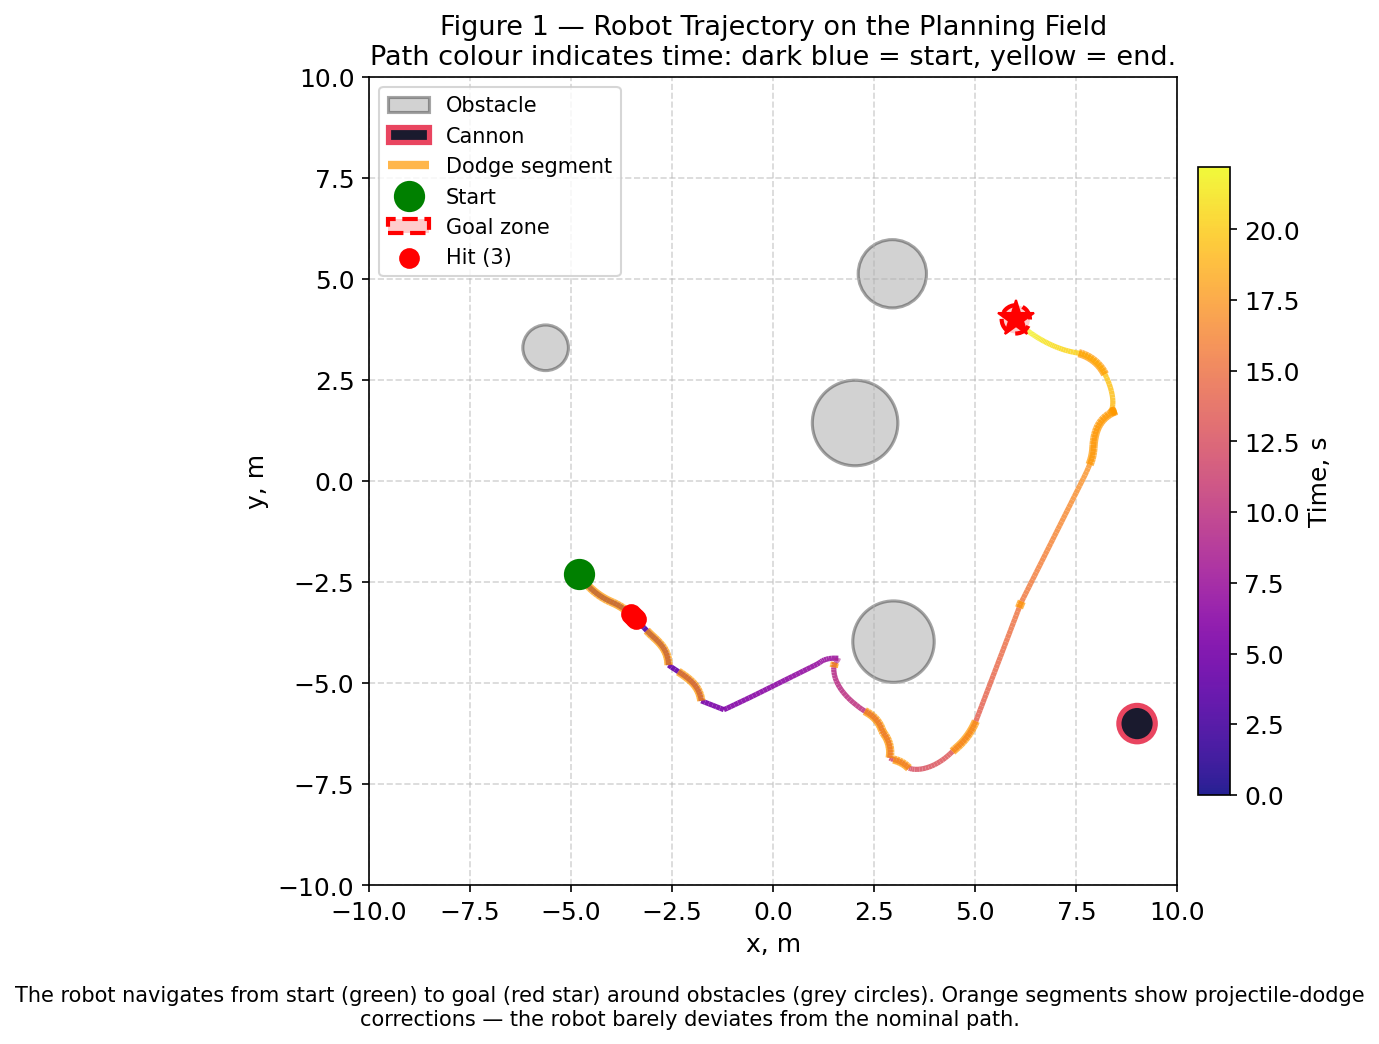
\includegraphics[width=0.85\textwidth]{figures/01_trajectory.png}
\caption{2D-траектория робота, цвет --- время. Видны обходы препятствий
         и отклонения при уклонении от снарядов.}
\label{fig:trajectory}
\end{figure}

\begin{figure}[H]
\centering
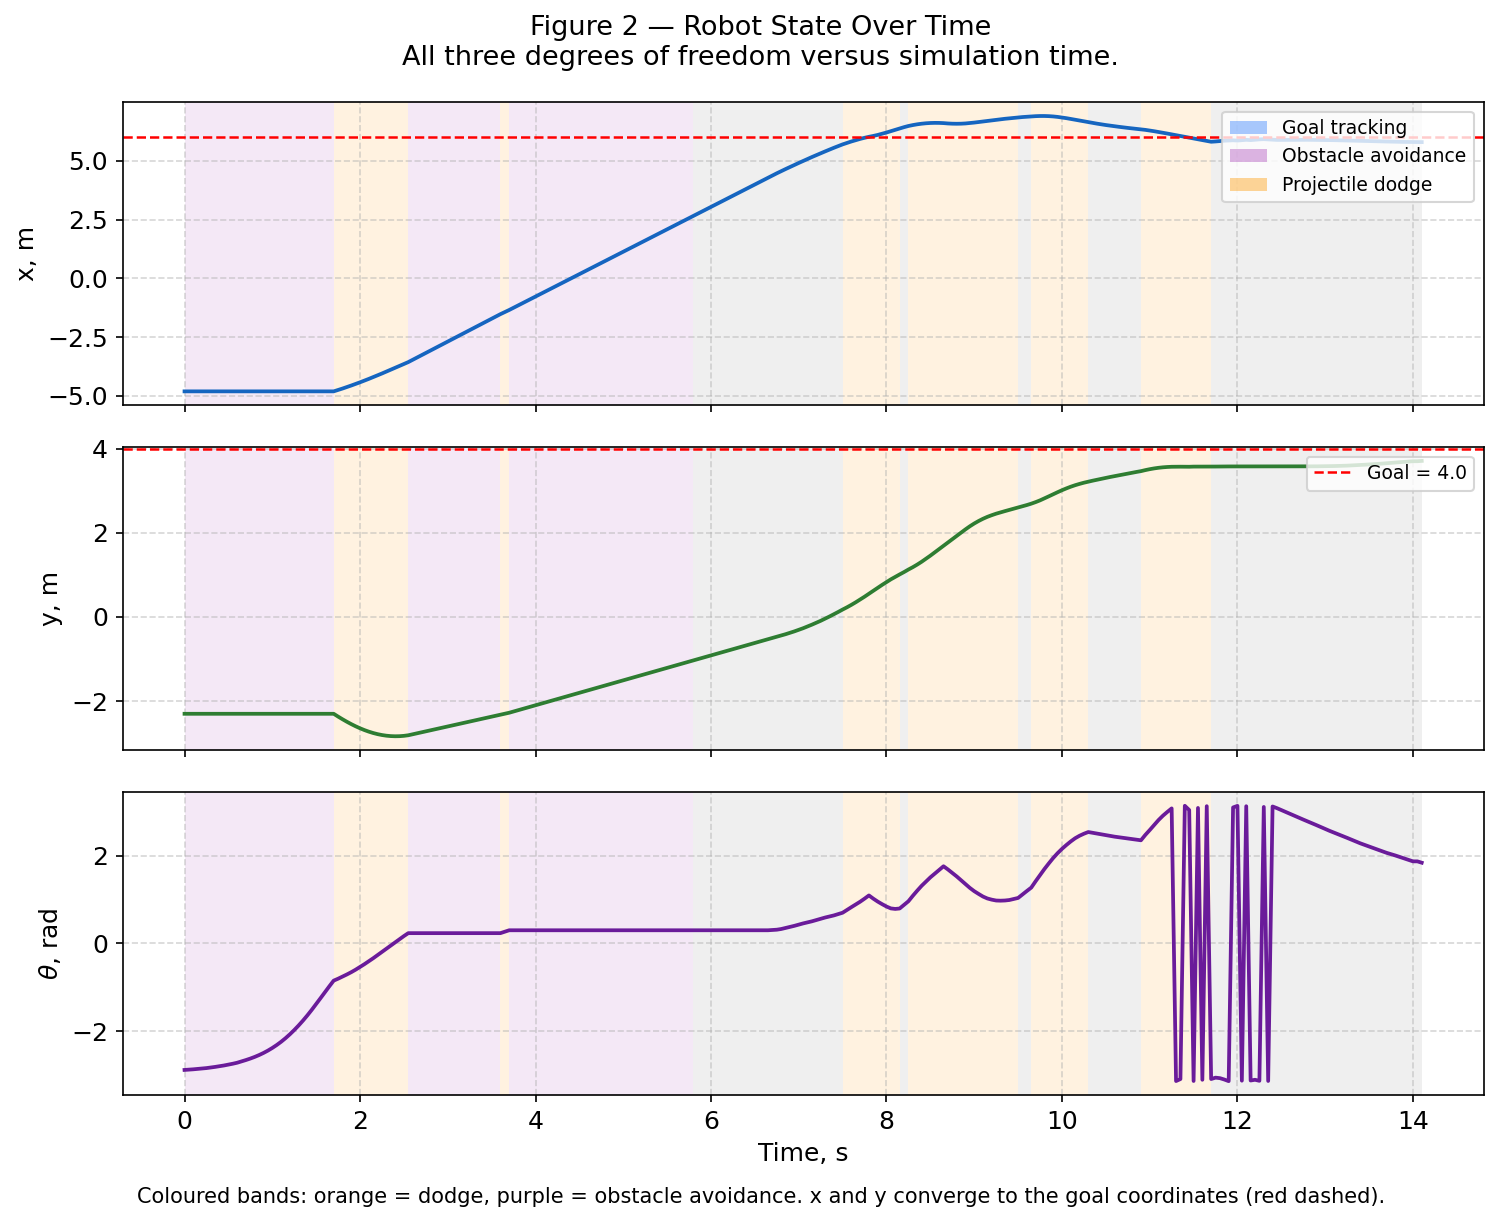
\includegraphics[width=0.85\textwidth]{figures/02_state_trajectories.png}
\caption{Временны\'{e} ряды $x(t)$, $y(t)$, $\theta(t)$.}
\label{fig:states}
\end{figure}

\begin{figure}[H]
\centering
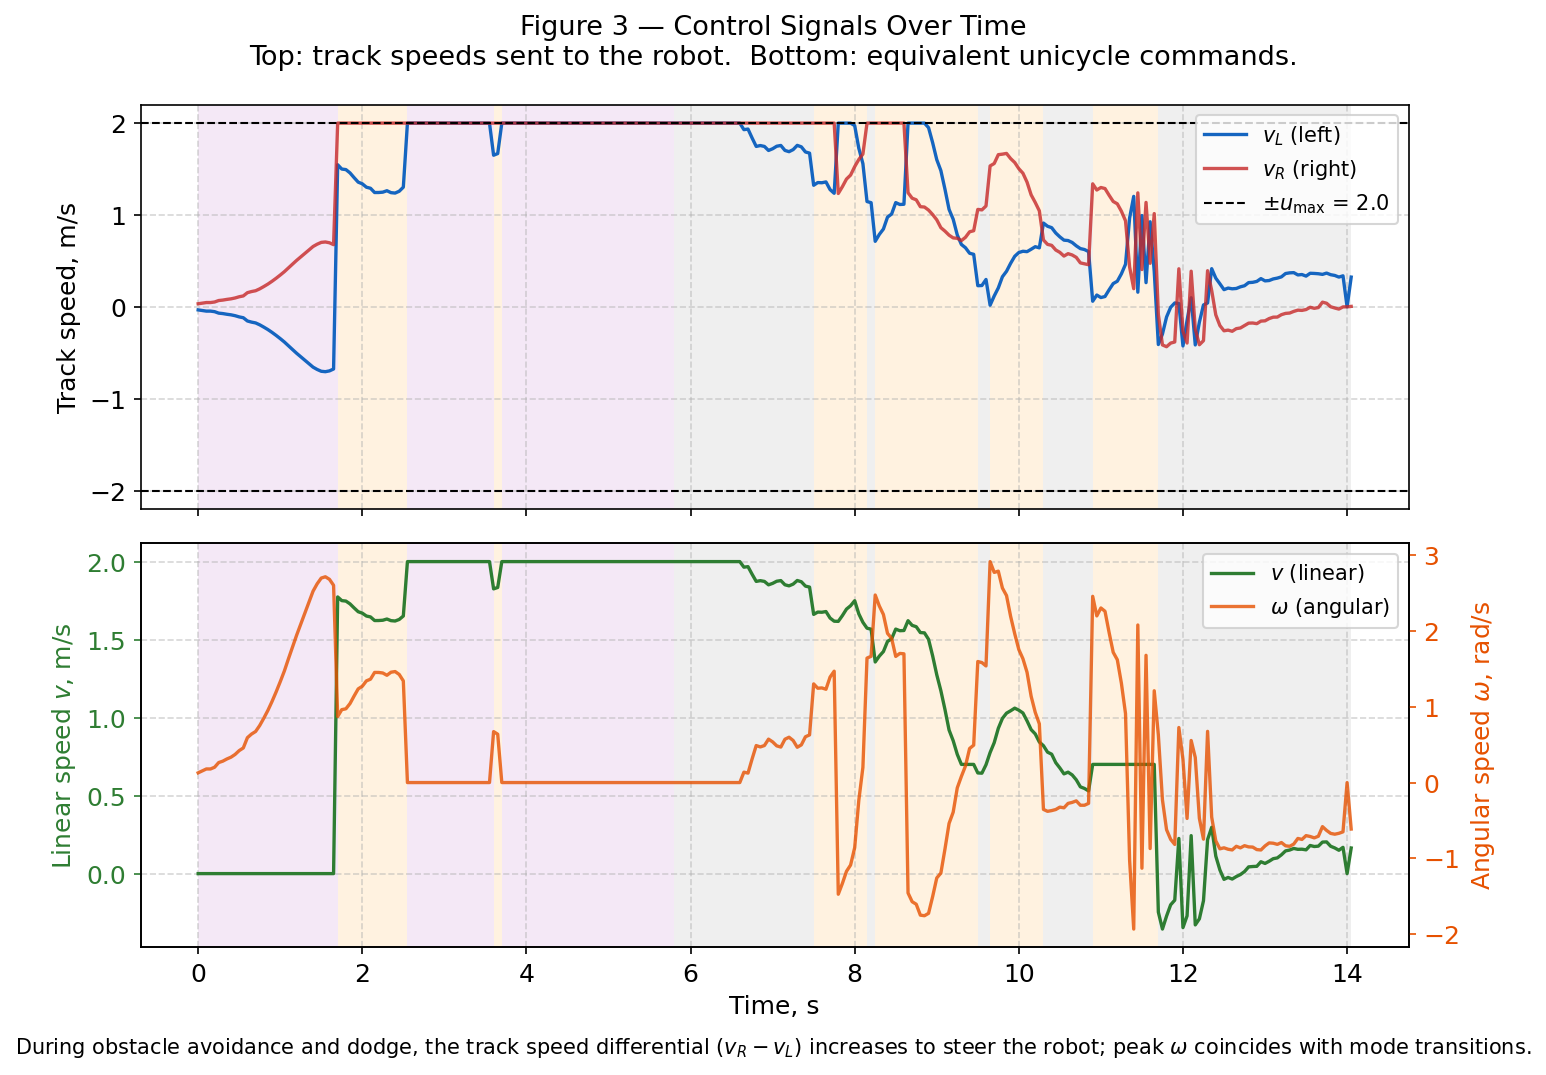
\includegraphics[width=0.85\textwidth]{figures/03_control_signals.png}
\caption{Управляющие сигналы: гусеничные скорости $v_L(t)$, $v_R(t)$ и
         unicycle-координаты $v(t)$, $\omega(t)$.  Видны насыщения при $\pm 2$ м/с
         и импульсы $\omega$ при dodge.}
\label{fig:controls}
\end{figure}

\begin{figure}[H]
\centering
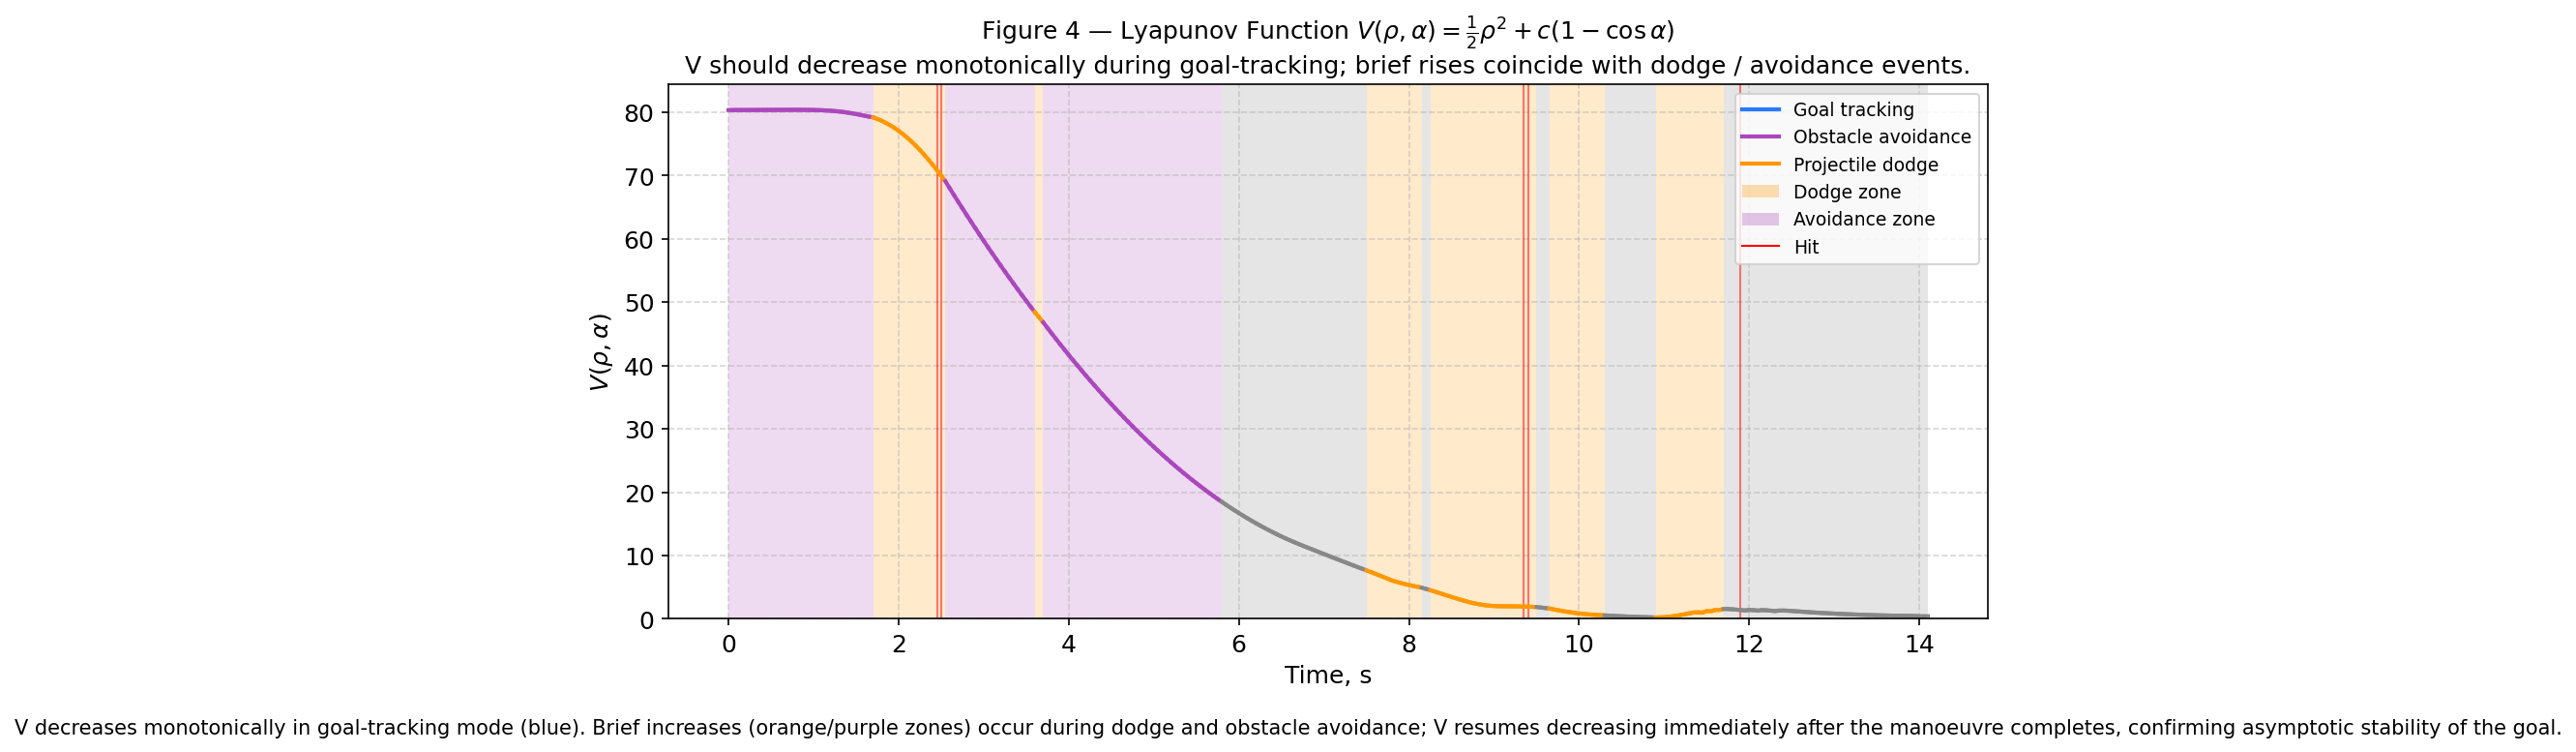
\includegraphics[width=0.85\textwidth]{figures/04_lyapunov.png}
\caption{Функция Ляпунова $V(t)$ с аннотацией режимов контроллера.  Монотонное
         убывание в goal-tracking; кратковременные подъёмы при obstacle avoidance
         и dodge.}
\label{fig:lyapunov}
\end{figure}

\begin{figure}[H]
\centering
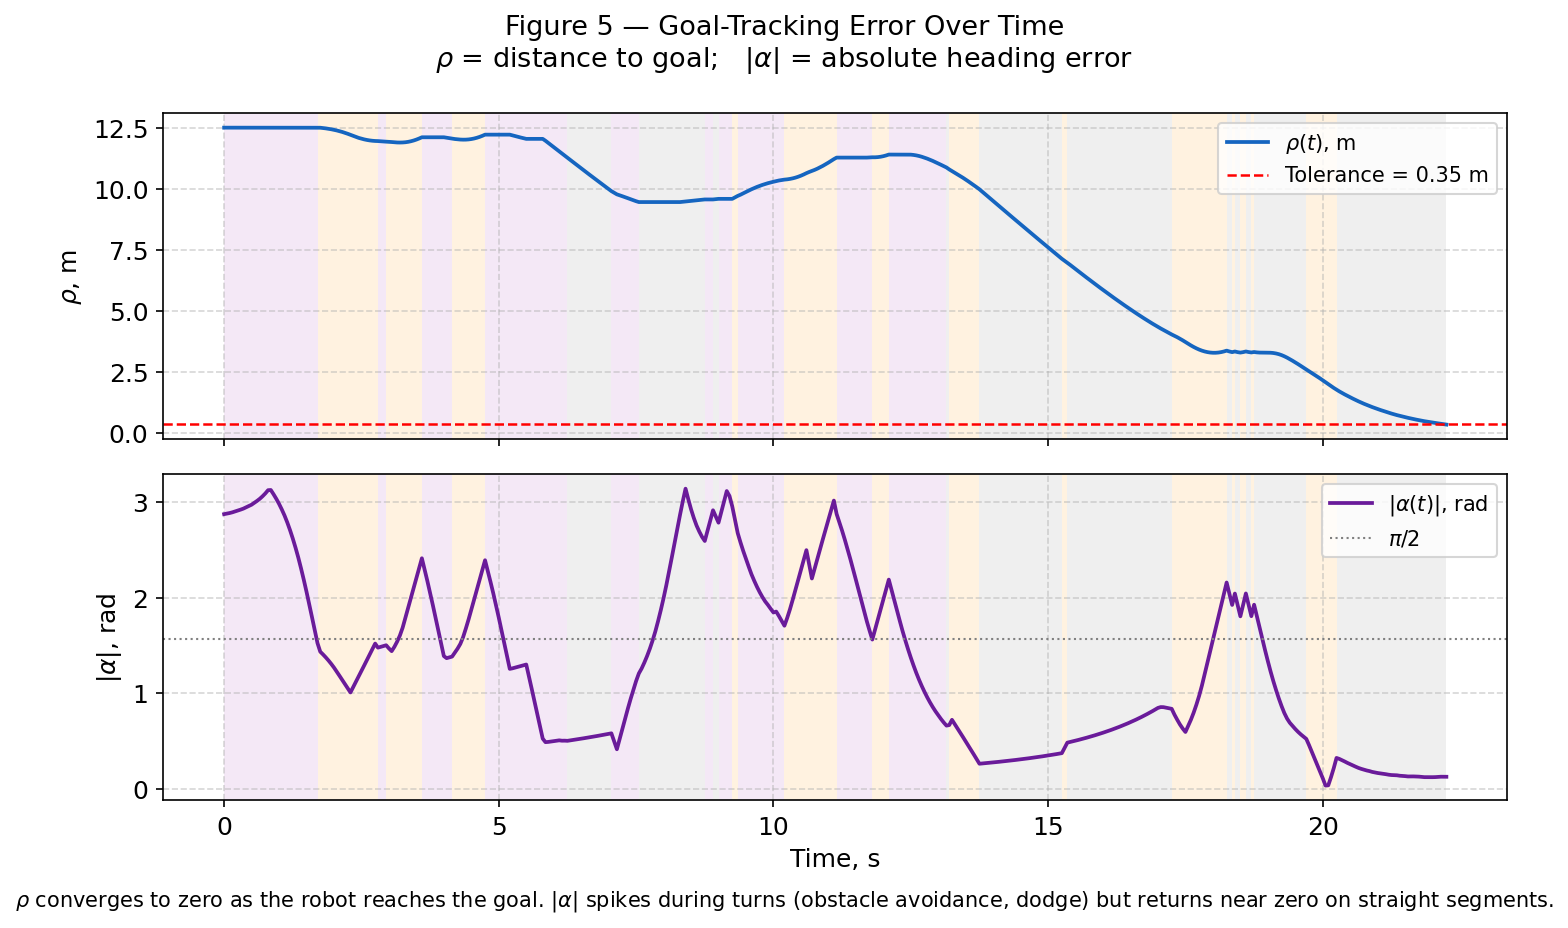
\includegraphics[width=0.85\textwidth]{figures/05_error_metrics.png}
\caption{Метрики ошибки: $\rho(t)$ (расстояние до цели) и $|\alpha(t)|$ (ошибка
         курса).  Обе стремятся к нулю.}
\label{fig:errors}
\end{figure}

\begin{figure}[H]
\centering
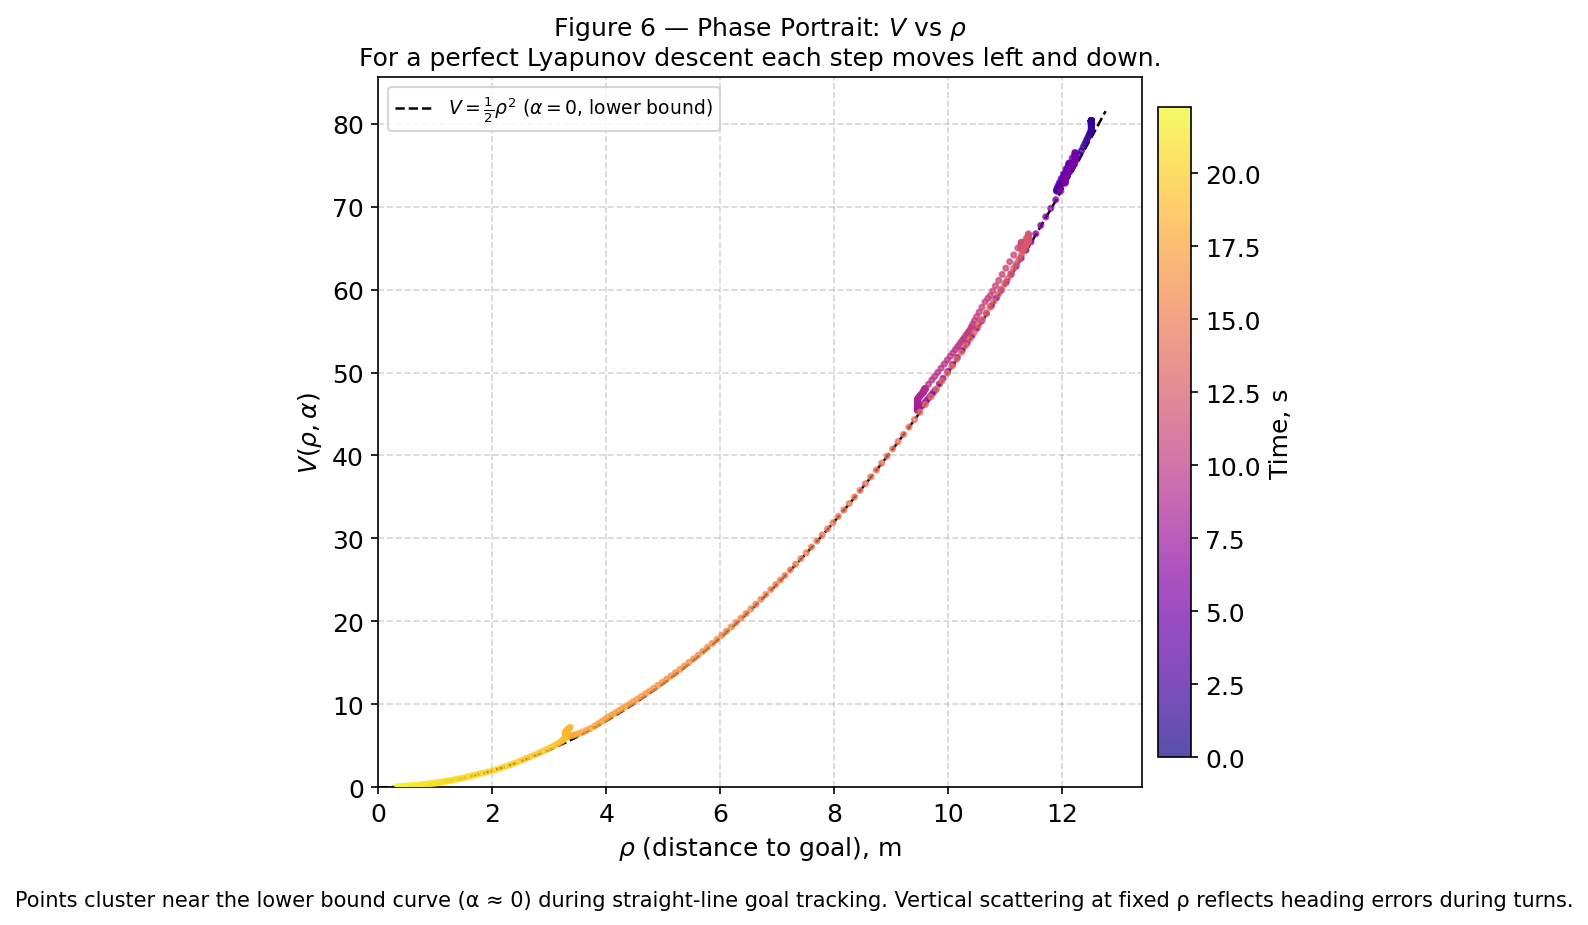
\includegraphics[width=0.85\textwidth]{figures/06_phase_portrait.png}
\caption{Фазовый портрет $V$ vs $\rho$.  Петли при obstacle avoidance, но общий
         тренд $\to 0$.}
\label{fig:phase}
\end{figure}

\subsection{Ограничения}

\begin{enumerate}
  \item \textbf{Нет формальной гарантии устойчивости при dodge:}  Доказательство
        $\dot{V} \le 0$ применяется к smooth goal-tracking.  При dodge контроллер
        добавляет $\Delta\omega$, и $V$ может кратковременно расти.

  \item \textbf{Реактивный, не глобально оптимальный обход:}  Tangent-waypoint
        планировщик может требовать нескольких waypoints для узких проходов и
        застревать на очень плотных конфигурациях.

  \item \textbf{Попадания снарядов:}  С текущими параметрами робот получает
        небольшое число попаданий за прогон.  Более агрессивный lookahead или
        предиктивное планирование пути снизили бы это число.

  \item \textbf{Голономное допущение при dodge:}  Направление уклонения вычисляется
        в предположении мгновенной реакции.  При малой скорости или большой ошибке
        курса реальный зазор может быть меньше предсказанного.
\end{enumerate}

% ====================================================================
\section{Алгоритм (псевдокод)}\label{sec:algorithm}
% ====================================================================

\begin{lstlisting}[language=Python, caption={Главный цикл симуляции}, label={lst:main}]
INPUT:  s0, goal g, obstacles O, cannon_config, noise_config
OUTPUT: state trajectory, control history, Lyapunov history

sim   <- TrackedRobotSim(s0)
ctrl  <- LyapunovController(g, O)
cannon <- Cannon(Poisson rate)
filtered_state <- s0

FOR k = 0, 1, ..., N-1:

  1. CANNON UPDATE
     new_proj <- cannon.update(dt, t_k, robot_pos)
     advance all live projectiles by dt
     remove expired / out-of-bounds projectiles

  2. COLLISION DETECTION
     sim.record_projectile_snapshot(projectiles)

  3. MEASUREMENT
     noisy_state <- state + N(0, sigma^2)
     filtered_state <- EMA(noisy_state, filtered_state)

  4. CONTROL (priority order)
     a. IF rho < eps_goal     -> u = 0        (STOP)
     b. ELIF threat detected  -> DODGE         (angular bias)
     c. ELIF obstacle blocks  -> AVOIDANCE     (waypoint)
     d. ELSE                  -> GOAL TRACKING (Lyapunov)
     Convert (v, omega) -> (v_L, v_R), clip

  5. STEP SIMULATOR
     state <- sim.step(u)

  6. IF rho(true_state, g) < tolerance -> BREAK
\end{lstlisting}

% ====================================================================
\section*{Заключение}
% ====================================================================

В данном проекте реализовано Ляпунов-управление гусеничным роботом с
аналитически доказанной асимптотической устойчивостью целевого положения
равновесия.  Система дополнена реактивным обходом статических препятствий
(tangent waypoints), уклонением от снарядов (angular bias injection на основе
CPA-анализа) и EMA-фильтрацией зашумлённых измерений.  Экспериментальные
результаты подтверждают сходимость $V \to 0$ и робастность к шуму и внешним
воздействиям.

\begin{thebibliography}{9}
\bibitem{aicardi1995}
  M.~Aicardi, G.~Casalino, A.~Bicchi, A.~Balestrino,
  \emph{Closed loop steering of unicycle-like vehicles via Lyapunov techniques},
  IEEE Robotics \& Automation Magazine, vol.~2, no.~1, pp.~27--35, 1995.

\bibitem{khalil2002}
  H.~K.~Khalil,
  \emph{Nonlinear Systems}, 3rd ed., Prentice Hall, 2002.

\bibitem{lavalle2006}
  S.~M.~LaValle,
  \emph{Planning Algorithms}, Cambridge University Press, 2006.
\end{thebibliography}

\end{document}
